
%
\section{VrtSecInclusive \label{sec:VSI} }
%

This section serves to generically document the VrtSecInclusive setup.
The performance in specific models will be discussed in the following sections.

%
%-------------------------------------------------------------------------------
\subsection{Introduction}
\label{sec:intro}
%-------------------------------------------------------------------------------

{\tt VrtSecInclusive}~\cite{} is an {\tt athena} package which offers reconstruction of displaced vertices from the given input {\tt xAOD::TrackParticle} container. The package was originally developed by Vadim Kostyukhin around 2004, who is also the developer of a generic vertex fitting core service {\tt VKalVrt}~\cite{} that {\tt VrtSecInclusive} bases on. Since Run 2, the package has been mostly maintained by Hideyuki Oide.

Traditionally, the main application of the package was inner detector material studies with hadronic interactions, and ATLAS has released three ID material papaers~\cite{} with utilising this package in Run~1 and Run~2. Lately, the package is also applied to various new physics searches that make use of displaced vertices as the signature in both SUSY and exotic searches. One reason of this is that the development of the package that had been used for such applications, {\tt RpvDispVrt} \cite{}, which was historically branched from {\tt VrtSecInclusive}, was discontinued. However, due to its historical primary target application of the package is somewhat different from these searches, several sub-optimal situations have been noticed through an application of the package to the SUSY DV+MET search and other ongoing analyses~\cite{}.

\begin{itemize}
  \item It is observed that the hit-pattern consistency requirement is not ideal when disabled modules are present at the closest outer layer than the vertex. The vertices are falsely identified to be killed, and producing an acceptance loss.
  \item Significant fraction of $R$-hadron vertices are reconstructed as split vertices. This is not favourable since it results in deterioration of the main signal discriminants, track multiplicity $N_{\rm track}$ and the vertex invariant mass $m_{\rm vtx}$.
\end{itemize}

Before production of {\tt DAOD\_RPVLL} dataset with {\tt athena} release {\tt 21}, general overhaul campaign of the package code structure was carried out, with adding new features to overcome the above issues. With these revisions, {\tt VrtSecInclusive} expands its capability in many aspects and is now expected to provide better performance. In addition, the code was refurbished to be as modern as the {\tt C++11/14} coding conventions, and the maintainability of the package has improved largely. This note describes the technical detail of features that the package offers, performance benchmarks as well as job properties that users can handle and its effect as user's reference.

%-------------------------------------------------------------------------------
\subsection{Algorithm}
\label{sec:structure}
%-------------------------------------------------------------------------------

\subsubsection{General notes on secondary vertexing}
Each track has a finite `thickness' represented by the track parameters covariance matrix, and a vertex can be formed when arbitrary two tracks share a common space within the tracking volume. For a given profile of track parameters, the probability of producing random combinatorial vertices is expected to roughly scale to $C(n,2)\propto {\cal O}(n^{2})$. In addition, the fraction of the volume which each track occupies within a given radius $r$ is proportional to ${\cal O}(r)/(\pi r^{2}\varDelta z)\propto {\cal O}(1/r)$, implying that the probability of random combinatorial vertexing should be proportional to ${\cal O}(1/r^{2})$ even without correlations between tracks. In addition, the track $d_{0}$ distribution has a very strong concentration at small $|d_{0}|$. In addition, the collision environment with high $\langle\mu\rangle$ increases the track density.

Therefore it is essential to effectively select seed tracks of interests and reject anything else, in order to suppress combinatorial fake vertices. For example, the SV algorithm used in $b$-tagging only uses tracks compatible with a seed jet. The algorithm described in this note, {\tt VrtSecInclusive}, does not have such phase space limitation, and it attempts to reconstruct as inclusive secondary vertices as possible. However due to the constraints described above, there are fundamental limitations especially for reconstruction efficiency at small radii within a few mm.

Typical applications of {\tt VrtSecInclusive} is reconstruction of the decays of \Kshort, hadronic interaction and hypothetical $R$-hadrons. For specific cases, {\tt VrtSecInclusive} might not be sufficiently powerful, and development or usage of other specialised vertexing might be recommended.

\subsubsection{Prerequisites}
It is required that the event contains the primary vertex ({\tt Vertex::PriVtx}) in the vertex container. Otherwise, the entire event is passed.

\subsubsection{Seed track selection}
The algorithm starts with selecting tracks from the specified {\tt xAOD::TrackParticleContainer}. The default used container is {\tt InDetTrackParticles} and the algorithm select seed tracks from it. Alternatively, options {\tt doSelectTracksFromMuons} and\\ {\tt doSelectTracksFromElectrons} job properties are equipped. If either of these two options is enabled, the algorithm does not use {\tt InDetTrackParticles} primarily, but it rather seeks candidate ID tracks linked from {\tt xAOD::Muon} or {\tt xAOD::Electron} objects. Note that {\tt doSelectTracksFromMuons} and {\tt doSelectTracksFromElectrons} can stand simultaneously, and hence it allows to reconstruct vertices of an $(e,\mu)$ pair for example.

This track selection step for vertex seeding is very important to keep the signal efficiency high but reducing the fake vertices rate as well as CPU time consumption, and in general a careful optimisation is required.

Several track selection functions are equipped in the package, and user can specify which selections to be applied by the job property. Each selection function has a common format of
\begin{scriptsize}
\begin{verbatim}
bool VrtSecInclusive::FUNCTION_NAME( const xAOD::TrackParticle* ) const
\end{verbatim}
\end{scriptsize}

and if the job property specifies to use the corresponding function, the function is registered to the list of requirements. For each track in the container, each cut function in the list is tried, and an array of booleans is created as the result. The track selection function only registers the track if all of these booleans are {\tt true}. The available selection functions are listed in Table \ref{tbl:trackSelection}.

\begin{description}
\item{{\tt selectTrack\_pTCut} (always enabled)}\\This function selects only tracks with having greater \pt than the user-specified threshold by the job property {\tt TrkPtCut}.
\item{{\tt selectTrack\_chi2Cut} (always enabled)}\\ This function selects only tracks with having smaller $\chi^{2}/N_{\rm dof}$ than the user-specified maximum threshold by the job property {\tt TrkChi2Cut}.
\item{{\tt selectTrack\_hitPattern} (always enabled)}\\ This function selects tracks which satisfy a hit pattern requirement configured by the user. Several options are available to flexibly optimise the track selection as follows.
  \begin{itemize}
  \item When the job property flag {\tt SAloneTRT} is \emph{disabled} (default: disabled), tracks which do not satisfy to have minimal numbers of \{ pixel hits, SCT hits, the sum of pixel and SCT hits, innermost pixel layer's hits \} (with each value specified by the job properties {\tt CutPixelHits}, {\tt CutSctHits}, {\tt CutSiHits}, {\tt CutBLayHits}, {\tt CutSharedHits} respectively) are rejected. In addition, tracks which have more shared hits than the user-specified value are rejected.
  \item When the job property flag {\tt doTRTPixCut} is enabled (default: disabled), tracks which do not have any TRT hits when the number of pixel hits are less than two are rejected.
  \item When there is no pixel hits, tracks do not have at least six SCT hits are rejected.
  \end{itemize}

\item{{\tt selectTrack\_hitPatternTight} (always enabled)}\\ This function selects tracks which satisfy an additional hit pattern requirement to {\tt selectTrack\_hitPattern} configured by the user.
  \begin{itemize}
  \item This filter is not activated when the track \pt is greater than 20 \GeV. The main purpose of having this tight selection is to reduce the density of tracks which could produce many fake vertices.
  \item For the low-\pt tracks, it is required to have the number of SCT hits to be at least the user-specified value (default: 7).
  \item for the low-\pt tracks within $|\eta|<1.6$, it is required to have the number of TRT hits to be at least the user-specified value (default: 20).
  \end{itemize}

\item{{\tt selectTrack\_notPVassociated} (default: {\tt true}; activated by {\tt do\_PVvetoCut}})\\This function rejects all tracks which are associated to the (hard-scatter) primary vertex or pileup vertices. There is no user-specified job property for this function.
\item{{\tt selectTrack\_d0Cut} (default: {\tt true}; activated by {\tt do\_d0Cut})}\\This function selects only tracks which satisfy the user-specified range of transverse impact parameter $|d_{0}|$ with respect to the beam spot. The min/max $d_{0}$ value is specified by {\tt a0TrkPVDstMinCut} and {\tt a0TrkPVDstMaxCut} respectively.
\item{{\tt selectTrack\_z0Cut} (default: {\tt true}; activated by {\tt do\_z0Cut})}\\This function selects only tracks which satisfy the user-specified range of transverse impact parameter $|z_{0}|$ with respect to the beam spot, meaning that the $z$-position of the track which gives the transverse impact parameter $d_{0}$. The min/max $z_{0}$ value is specified by {\tt zTrkPVDstMinCut} and {\tt zTrkPVDstMaxCut} respectively.
\item{{\tt selectTrack\_d0errCut} (default: {\tt false}; activated by {\tt do\_d0errCut}})\\This function selects only tracks which satisfy the user-specified maximum value on the uncertainty of $d_{0}$. Practically it refers the $(0,0)$ component of the track parameter covariance matrix $\Sigma$ and applies a cut $\Sigma_{00} < \left(\sigma_{d_{0}}^{\rm max}\right)^{2}$. User can specify $\sigma_{d_{0}}^{\rm max}$ by the job property {\tt TrkA0ErrCut}.
\item{{\tt selectTrack\_z0errCut} (default: {\tt false}; activated by {\tt do\_z0errCut}})\\This function selects only tracks which satisfy the user-specified maximum value on the uncertainty of $z_{0}$. Practically it refers the $(1,1)$ component of the track parameter covariance matrix $\Sigma$ and applies a cut $\Sigma_{11} < \left(\sigma_{z_{0}}^{\rm max}\right)^{2}$. User can specify $\sigma_{z_{0}}^{\rm max}$ by the job property {\tt TrkZErrCut}.
\end{description}

Once the track passed all the required selections, then the variable {\tt is\_selected} is augmented to it. If the number of selected tracks is less than two, the algorithm ends. Also, if the number of selected tracks is larger than the user=specified limit (by the job property {\tt SelTrkMaxCutoff}, default: 50), the algorithm ends.


\begin{table}[t]
\caption{List of track selection function strategies in release {\tt 21}. The column ``default'' indicates the activation of the function by default at the level of the package, and not at the level of any job option.}
\centering
\begin{scriptsize}
\begin{tabular}{llll}
\hline
\hline
Function name & Description& default\\
\hline
{\tt selectTrack\_pTCut} & Apply the minimum $\pt$ requirement & true\\
{\tt selectTrack\_chi2Cut} & Apply the maximum track $\chi^{2}/N_{\rm dof}$ requirement & true\\
{\tt selectTrack\_hitPattern} & Apply the hit pattern requirement & true\\
{\tt selectTrack\_hitPatternTight} & Apply the tight hit pattern requirement & true\\
{\tt selectTrack\_notPVassociated} & Select only tracks which are not associated to primary/pileup vertices & false \\
{\tt selectTrack\_d0Cut} & Apply cut to $|d_{0}|$ wrt. beam spot & true\\
{\tt selectTrack\_z0Cut} & Apply cut to $|z_{0}|$& true\\
{\tt selectTrack\_d0errCut} & Apply cut to $d_{0}$ error & false\\
{\tt selectTrack\_z0errCut} & Apply cut to $z_{0}$ error & false\\
%{\tt selectTrack\_d0signifCut} & Apply cut to $d_{0}$ significance (not commissioned) & & false\\
%{\tt selectTrack\_z0signifCut} & Apply cut to $z_{0}$ significance (not commissioned) & & false\\
\hline
\hline
\end{tabular}
\end{scriptsize}
\label{tbl:trackSelection}
\end{table}%

\subsubsection{General on vertexing sequence}
After the seed track selection is over, the vertex reconstruction sequence starts. Each vertexing function has a format of 

\begin{scriptsize}
\begin{verbatim}
StatusCode VrtSecInclusive::FUNCTION_NAME( std::vector<WrkVrt>* workVerticesContainer )
\end{verbatim}
\end{scriptsize}

and the vector of temporary vertex object ({\tt WrkVrt}) is passed from one function to the next in a cascading manner. Practically this is done by storing the list of functions in a vector of function pointers:

\begin{scriptsize}
\begin{verbatim}
StatusCode VrtSecInclusive::initialize() {
  ...
  m_vertexingAlgorithms.emplace_back( make_pair( "extractIncompatibleTrackPairs", extractIncompatibleTrackPairs ) );
  m_vertexingAlgorithms.emplace_back( make_pair( "findNtrackVertices",            findNtrackVertices )            );
  m_vertexingAlgorithms.emplace_back( make_pair( "rearrangeTracks",               rearrangeTracks)                );
  ...
}

...

StatusCode VrtSecInclusive::execute() {
  ...
  for( auto itr = m_vertexingAlgorithms.begin(); itr!=m_vertexingAlgorithms.end(); ++itr ) {
      
      auto& name = itr->first;
      auto alg   = itr->second;
      
      // workVerticesContainer is std::vector<WrkVrt>*
      ATH_CHECK( (this->*alg)( workVerticesContainer ) );
      ...
  }
  ...
}
\end{verbatim}
\end{scriptsize}


\subsubsection{Di-track vertex finding}\label{sec:ditrack}

The vertex forming starts with attempting to form vertices for all $C(n,2)$ combinations of pair-tracks from the selected tracks then the algorithm attempts to form the vertex. This step consumes the dominant CPU time. In order to reduce the fake vertices yield and to save the CPU time consumption, the following pre-selections are applied:

\begin{itemize}
\item if $|d_{0}|$ of either of the pair tracks is less than the user-specified value (job property:\\ {\tt twoTrkVtxFormingD0Cut}), the pair is rejected;
\item then the rough initial vertex position is estimated in an analytical manner by {\tt VKalVrtFitFast}. If the transverse radius of the initial vertex position is greater than 563 mm\footnote{Corresponding to the inner surface of the TRT.}, the pair is rejected. Next the impact parameter of the two tracks with respect to the initial vertex position, $(d_{0}^{\rm init}, z_{0}^{\rm init})$ is calculated. If either of $|d_{0}^{\rm init}|$ (\,$|z_{0}^{\rm init}|$\,) is greater than 100 mm (50 mm), then the pair is rejected. Figure \ref{fig:initVertexDisp} shows the distribution of $|d_{0}^{\rm init}|$ and $|z_{0}^{\rm init}|$ as a function of vertex $r$ and $z$ (respectively) for the case the precision vertex fitting obtained the vertex.
\end{itemize}

\begin{figure}[t]
\begin{center}
\subfigure[x]{ 
  \label{fig:initVertexDispD0} 
  \includegraphics[width=0.48\textwidth]{figures/initVertexDispD0_mc15_13TeV_402735}
}
\subfigure[]{ 
  \label{fig:initVertexDispZ0} 
  \includegraphics[width=0.48\textwidth]{figures/initVertexDispZ0_mc15_13TeV_402735}
}
\caption{Distribution of \subref{fig:initVertexDispD0} $d_{0}^{\rm init}$ and \subref{fig:initVertexDispZ0} $z_{0}^{\rm init}$ as a function of vertex $r$ and $z$ (respectively) for the case the precision vertex fitting obtained the vertex. The entries in $z$-axis is normalised for each $y$-axis bin.}
\label{fig:initVertexDisp}
\end{center}
\end{figure}

It is measured that the latter item above is effective to reduce the CPU time consumption of the by around factor 5.

Only for the track pairs which pass the above criteria, the precision vertex fitting, {\tt VKalVrtFit}, is applied, and further vertex selection continues. If the vertex $\chi^{2}/N_{\rm dof}$ is larger than the user-specified threshold, it is dropped\footnote{In {\tt VrtSecInclusive}, $N_{\rm dof} \equiv 2\times N_{\rm track} - 3$. Contrary to the adaptive vertex fitting, all tracks have an equal weight.}.

\pagebreak
Some additional filters described as follows can be optionally applied in this stage.
\paragraph{Vertex position vs.~momentum requirement}
This option is activated by the user-specified job property {\tt doPVcompatibilityCut} (default:~{\tt true}). Several kinematic cuts are applied using the vertex pointing vector $\vec{r} = \vec{r}(r_{v}, z_{v},\phi_{v})$, which is defined as the relative position of the fitted vertex with respect to the hard-scatter primary vertex:

\begin{itemize}
\item the relative azimuthal angle difference between $\vec{r}$ and each of the track parameters $\phi^{(1,2)}$, $\varDelta\phi^{(1,2)}\equiv \phi^{(1,2)}-\phi_{\vec{r}}$ is calculated. If either of the track does not satisfy $\cos(\varDelta\phi^{(j)})< -0.8$, the vertex is rejected;
\item the vectorial sum of the momentum of the two tracks $\vec{p}^{\rm\,sum} = \vec{p}^{\rm\,sum}(p_{\rm T}^{\rm\,sum}, \eta^{\rm sum}, \phi^{\rm sum})$ is calculated. If the cosine of the angle between $\vec{p}_{\rm T}^{\rm\,sum}$ and the transverse component of $\vec{r}$, i.e. $\cos(\phi^{\rm sum}-\phi_{v})$ is less than $-0.8$, then the vertex is rejected. Figure~\ref{fig:vPosMomAngDistT} shows the distribution of $\cos(\phi^{\rm sum}-\phi_{v})$ as a function of transverse distance of the vertex from the origin for a case of SUSY long-lived $R$-hadon decays with $(m_{\gluino}, m_{\tilde{\chi}}) = (2000, 100)~{\rm GeV}$ and $\tau_{\gluino} = 1~{\rm ns}$ and for data;
\item the vertex is rejected if $\vec{r}\cdot(\vec{p}^{\rm\,sum}/|\vec{p}^{\rm \,sum}|) < K$ where $K$ is usually a negative value (default: $-20~{\rm mm}$; specified by the job property {\tt PVcompatibilityCut}). Kinematically this rejects too-negative correlation between $\vec{r}$ and $\vec{p}$, expecting that the decay product is expected to fly to outer direction. This option was hard-coded in release {\tt 20.7}, but from release {\tt 21} this is configurable as well as the threshold value. Figure~\ref{fig:vPosDist} shows the distribution of $\vec{r}\cdot(\vec{p}^{\rm\,sum}/|\vec{p}^{\rm \,sum}|)$ as a function of transverse distance of the vertex from the origin for a case of SUSY long-lived $R$-hadon decays with $(m_{\gluino}, m_{\tilde{\chi}}) = (2000, 100)~{\rm GeV}$ and $\tau_{\gluino} = 1~{\rm ns}$ and for data.
\end{itemize}


\begin{figure}[t]
\begin{center}
\subfigure[{\tt mc15\_13TeV.402735}]{ 
  \label{fig:vPosMomAngDistT_mc15_13TeV_402735} 
  \includegraphics[width=0.48\textwidth]{figures/vPosMomAngDistT_mc15_13TeV_402735}
}
\subfigure[{\tt data16\_13TeV.00310249}]{ 
  \label{fig:vPosMomAngDistT_data} 
  \includegraphics[width=0.48\textwidth]{figures/vPosMomAngDistT_data}
}
\caption{Distribution of $\vec{r}\cdot\vec{e}_{p}$ for \subref{fig:vPosMomAngDistT_mc15_13TeV_402735} an $R$-hadron MC simulation and \subref{fig:vPosMomAngDistT_data} for data. The entries in $z$-axis is normalised for each $x$-axis bin.}
\label{fig:vPosMomAngDistT}
\end{center}
\end{figure}

\begin{figure}[t]
\begin{center}
\subfigure[{\tt mc15\_13TeV.402735}]{ 
  \label{fig:vPosDist_mc15_13TeV_402735} 
  \includegraphics[width=0.48\textwidth]{figures/vPosDist_mc15_13TeV_402735}
}
\subfigure[{\tt data16\_13TeV.00310249}]{ 
  \label{fig:vPosDist_data} 
  \includegraphics[width=0.48\textwidth]{figures/vPosDist_data}
}
\caption{Distribution of $\vec{r}\cdot\vec{e}_{p}$ for \subref{fig:vPosDist_mc15_13TeV_402735} an $R$-hadron MC simulation and \subref{fig:vPosDist_data} for data. The entries in $z$-axis is normalised for each $x$-axis bin.}
\label{fig:vPosDist}
\end{center}
\end{figure}


\paragraph{Hit-pattern consistency check}
          {\tt xAOD::TrackParticle} has a variable {\tt hitPattern} which is an array of booleans with each of them representing the presence of the hit on the track for the corresponding pixel or SCT layer. If the calculated vertex is real, the constituent track should satisfy the hit pattern that is consistent with the causality of the given vertex position and the track parameter. If the hit-pattern check flag is enabled (default:{\tt true}), the track's hit pattern is required to be consistent with the expected hit pattern. Two algorithms are implemented, and the user can select it.
          
\begin{figure}[t]
\begin{center}
\subfigure[]{ 
  \label{fig:HadInt:fakeRejScheme1} 
  \includegraphics[width=0.48\textwidth]{figures/fakeRejectionScheme1}
}
\subfigure[]{ 
  \label{fig:HadInt:fakeRejScheme2} 
  \includegraphics[width=0.48\textwidth]{figures/fakeRejectionScheme2}
}
\caption{Schematic illustration of the \emph{classical} fake tracks rejection. \subref{fig:HadInt:fakeRejScheme1} The vertex is between the two layers of B-Layer and Layer-1 sensors. The tracks of the reconstructed secondary vertex must not have hits on the layers inner than the vertex radius (i.e.~IBL and B-Layer), and must have hits on the closest layer outside the vertex (i.e.~Layer-1). 
\subref{fig:HadInt:fakeRejScheme2} The vertex is close to the Pixel B-Layer sensors. 
In this example where the vertex is just inside the B-Layer, the tracks are not allowed to have hits on the IBL but may have hits on the B-Layer, and must have hits on the Layer-1.
Analogous requirements are made on vertices close to the other layers.
}
\label{fig:fakeRejScheme}
\end{center}
\end{figure}


\begin{enumerate}
\item \emph{Classical}: The algorithm classifies the vertex into multiple detector regions, and the each region has a hard-coded hit-pattern requirement for the track. For example, if the vertex is located between the pixel IBL and B-Layer, the tracks are \emph{forbidden} to have hits in IBL and they are \emph{required} to have hits in B-Layer. If the vertex position is close to senstive layers, such a requirement is relaxed, as illustrated in Figure~\ref{fig:fakeRejScheme}. The \emph{Classical} hit-pattern requirement is a simple and fast implementation, but it has some shortcomings.

One major problem is that the algorithm is agnostic of disabled modules, and it kills the vertices when the closest outer module is disabled and hits are missing there.

\item \emph{ExtrapolationAssist} (recommended): The same algorithm as \emph{Classical} runs, but the used hit pattern is complemented by the information of disabled modules by the track extrapolator. The track parameter is extrapolated along the momentum direction up to the end of the outermost SCT layer, then the disabled modules along the path are extracted. The logical {\tt OR} of the recorded hit pattern of the track, {\tt R}, and the disabled module pattern, {\tt D}, i.e. {\tt (R|D)} is used in the same algorithm as \emph{Classical}.

\item \emph{Extrapolation} (not yet fully commissioned - not recommended yet):  The other problem of the \emph{Classical} approach is that such classification is not well-defined when the vertices are near to the boundary between the barrel and endcap regions, and no selection is applied for vertices other than the barrel region. In order to improve such a situation, a new algorithm that employs the track extrapolator is implemented, as illustrated in Figure~\ref{fig:extrapolation}. 

In this method, the track extrapolation is made using the given track parameter, and it calculates the array of pixel and SCT module identifiers and the expected hit position from the perigee to the outer boundary of the inner detector volume. These array of expected hit positions, $\{P_{i}\}~(i=0, 1, 2,\cdots)$, where the index $i$ is labelled from the perigee to outer radii, can be compared to the vertex position $V$ as follows:
  \begin{itemize}
  \item If $P_{i}$ is inner than $V$, then the vector $\overrightarrow{P_{i}V}$ and the vector $\overrightarrow{P_{i}P_{i+1}}$ should direct the same orientation, i.e. the inner product $(\overrightarrow{P_{i}V}\cdot\overrightarrow{P_{i}P_{i+1}})$ is expected to be positive. Simultaneously, the transverse radius of the vertex must be outer than $P_{i}$. If this is the case, $P_{i}$ is not expected to have hit record.
  \item On the contrary, if the inner product $(\overrightarrow{P_{i}V}\cdot\overrightarrow{P_{i}P_{i+1}})$ is negative, the hit is expected to be present. Simultaneously, the transverse radius of the vertex must be inner than $P_{i}$. At this stage, the algorithm can ask to the detector condition service if the corresponding module is \emph{active} for the given dataset when the condition service is properly configured\footnote{This is automatically done when the algorithm runs in {\tt Reco\_tf.py} from ESD to AOD.}. In this way, disabled modules are taken into account properly.
  \item When a contradiction to the above conditions is detected, e.g.~$(\overrightarrow{P_{i}V}\cdot\overrightarrow{P_{i}P_{i+1}})>0$ when the transverse radius of the vertex is outer than $P_{i}$, it indicates that the vertex is reconstructed along the opposite $\phi$-direction to the track's outgoing direction, which is possible to happen. When this is detected, such vertices are rejected from candidates.
  \end{itemize}
  With this procedure, the extrapolation can reconstruct the expected hit pattern \emph{under the assumption of that the given vertex position is real}. Then this pattern is directly compared to the actually-recorded hit pattern. If the location of the first two innermost layers are identical between the expected and recorded hit patterns, the track is flagged as good. The vertex is rejected if either of the two tracks is not flagged as good.
\end{enumerate}

Generally, the \emph{extrapolation} option should provide more accurate hit-pattern consistency check.

\begin{figure}[t]
\begin{center}
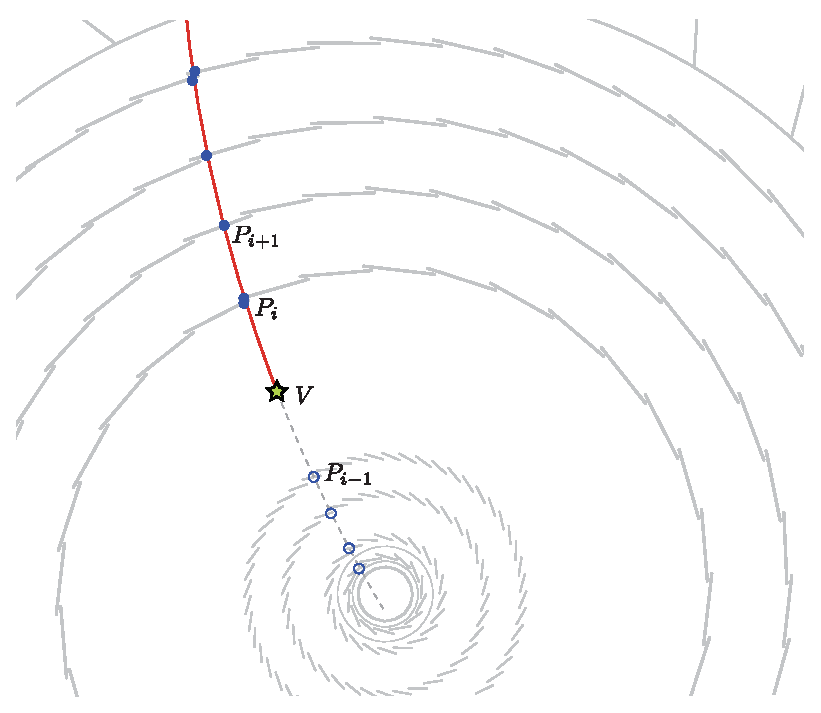
\includegraphics[width=0.5\textwidth]{figures/extrapolation}
\caption{Illustration of determining the expected hit-pattern using the track extrapolator.}
\label{fig:extrapolation}
\end{center}
\end{figure}



\subsubsection{Forming $n$-track vertices}
From the di-track vertexing algorithm described above, the collection of $C(n,2)$ track pairs are classified into two groups; the ones that satisfy the selection criteria, referred to as the \emph{compatible track pairs} and others, referred to as the \emph{incompatible track pairs} hereafter.

The approach that {\tt VrtSecInclusive} takes focuses on the incompatible track pairs rather than compatible track pairs. Here, the term incompatible means that the two-track pair is not able to form a vertex with a required quality. The list of incompatible track pairs in the event is represented as a graph like Figure~\ref{fig:incomp} (center) where the nodes (edges) represent tracks (incompatible pairs). The problem of finding $n$-track vertices is to find out sets of tracks in which the constituent tracks are all compatible each other. This problem can be translated as follows -- find the combination of nodes in the graph that achieves to remain only fully-isolated nodes when they are removed from the graph. In the example of the case in Figure~\ref{fig:incomp}, the solutions are removal of tracks $(3,4,5,6)$ and $(1,2,6)$. The remaining isolated tracks are regarded as the candidate $n$-track vertices and they are fitted as one vertex. Bad-quality vertices or vertices that are fully inclusive of other vertices are removed.

\begin{figure}[t]
\begin{center}
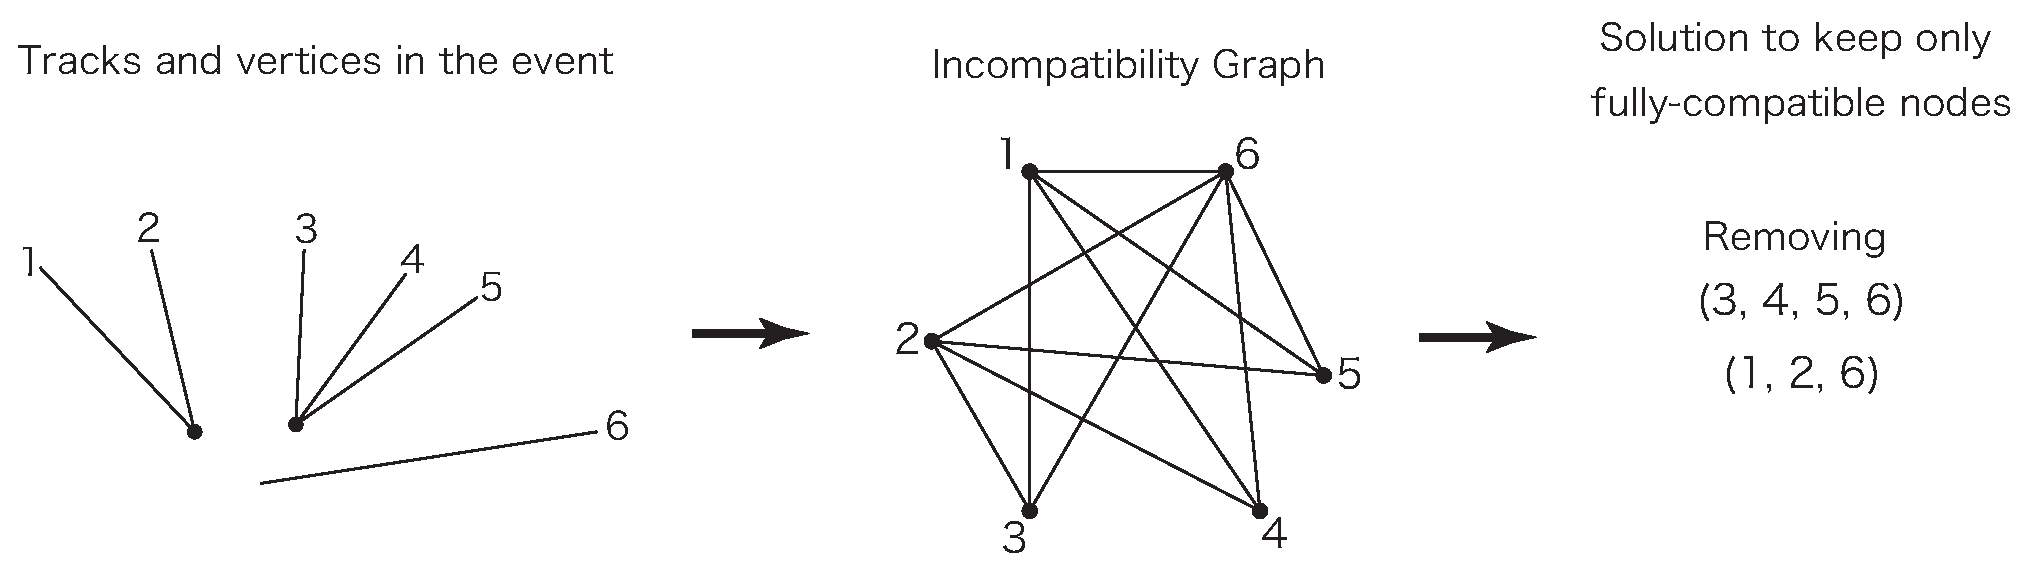
\includegraphics[width=1.0\textwidth]{figures/incomp}
\caption{An example of finding $n$-track vertices using the incompatibility graph. Left: layout of tracks and vertices in the event; Center: the incompatibility graph is formed by connecting two tracks when the di-track vertices are judged as incompatible; Right: finding out the set of tracks that are fully compatible each other.}
\label{fig:incomp}
\end{center}
\end{figure}


While the above method with the incompatible graph effectively works to form $n$-track vertices for relatively small multiplicity and all tracks from the same real vertex are compatible, the number of solutions may explode when the track multiplicity from the displaced vertex is very large and a fraction of track pairs is not compatible. Such a probability is expected to roughly increase with ${\cal O}(N_{\rm track}^{2})$. The second approach to form $n$-track vertices is {\it clustering} vertices as a simple and rapid algorithm. In this approach, the compatible track pairs are merged if their positions are closer than $1~{\rm mm}$. This second approach was implemented in the code but not commissioned yet, and still the incompatible graph approach is always used.

\subsubsection{Re-arrangement of tracks and vertex merging}
After $n$-track vertex finding using the incompatibility graph, a track may be compatible with multiple vertices, as illustrated in Figure~\ref{fig:rearrange}. In this case, the track index 3 is shared by two different vertices, and there is an ambiguity to which vertex this track should be associated. Since {\tt VrtSecInclusive} allows a track to be maximally associated to one secondary vertex, such ambiguity needs to be resolved. This step is referred to as \emph{re-arrangement}.

For each used track, the algorithm lists up all vertices which share it. The track that has the maximum shared vertices is identified. Subsequently, the goodness of association of the track to the shared vertices are asked, and the vertex with the worst goodness ($\chi^{2}$ per track) is identified. If the worst $\chi^{2}$ per track is larger than the specified threshold, then the track is removed from the vertex and repeat the sequence. Otherwise, the significance of the distance between vertices that share the track of interest as well as the number of shared tracks is measured, and if the significance is smaller than the specified threshold, or at least two tracks are shared, the two vertices are merged. If no vertices to be merged is found for the track of interest, in order to resolve the ambiguity, the track is detached from the worst-associated vertex. The same procedure repeats from the beginning until no shared tracks remain.

\begin{figure}[t]
\begin{center}
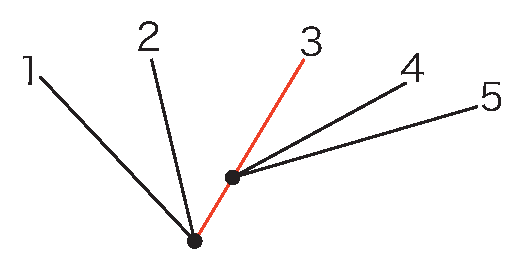
\includegraphics[width=0.47\textwidth]{figures/rearrange}
\caption{An example of track sharing by multiple vertices.}
\label{fig:rearrange}
\end{center}
\end{figure}

\subsubsection{Optional vertex merging algorithms [new in {\tt r21}]}\label{sec:merging}
It was observed in release {\tt 20.7} DV+MET analysis that some fraction of $R$-hadron vertices are split. In order to improve the situation, some new vertex-merging features have been added to {\tt VrtSecInclusive} in release {\tt 21}. The following options are mainly for vertices with a large track multiplicity.

\paragraph{Re-assembling}
The two-track vertex fitting may fall in a local-minimal solution, especially when the constituent tracks are approximately collinear. The position of such a vertex may be far away from the main vertex. In order to merge such vertices to the main vertex, the constituent tracks are extrapolated to the candidate main vertex. If \emph{all} of the constituent tracks are pointing to the candidate main vertex, then such a vertex is merged to the candidate vertex.

\paragraph{Suggested refitting}
Similar to the previous case that the vertex may be falling into a local-minimal solution, the vertex is attempted to refit with using the main vertex position as the initial suggested solution. If the vertex position after refitting is close enough to the main vertex, then the two vertices are merged.

\paragraph{Magnet merging}
Similar to the previous case that the vertex may be falling into a local-minimal solution, the vertex is attempted to refit, with adding one track from the candidate main vertex. This is repeated for all constituent tracks in the main vertex. If the refit vertex position is close enough to the main vertex, then the two vertices are merged.

\paragraph{Wild merging}
The two vertices are anyway attempted to merge, and if the refit result is close enough to the main vertex and the refit $\chi^{2}/N_{\rm dof}$ is satisfactory, the two vertices are merged.


%\begin{figure}[t]
%\begin{center}
%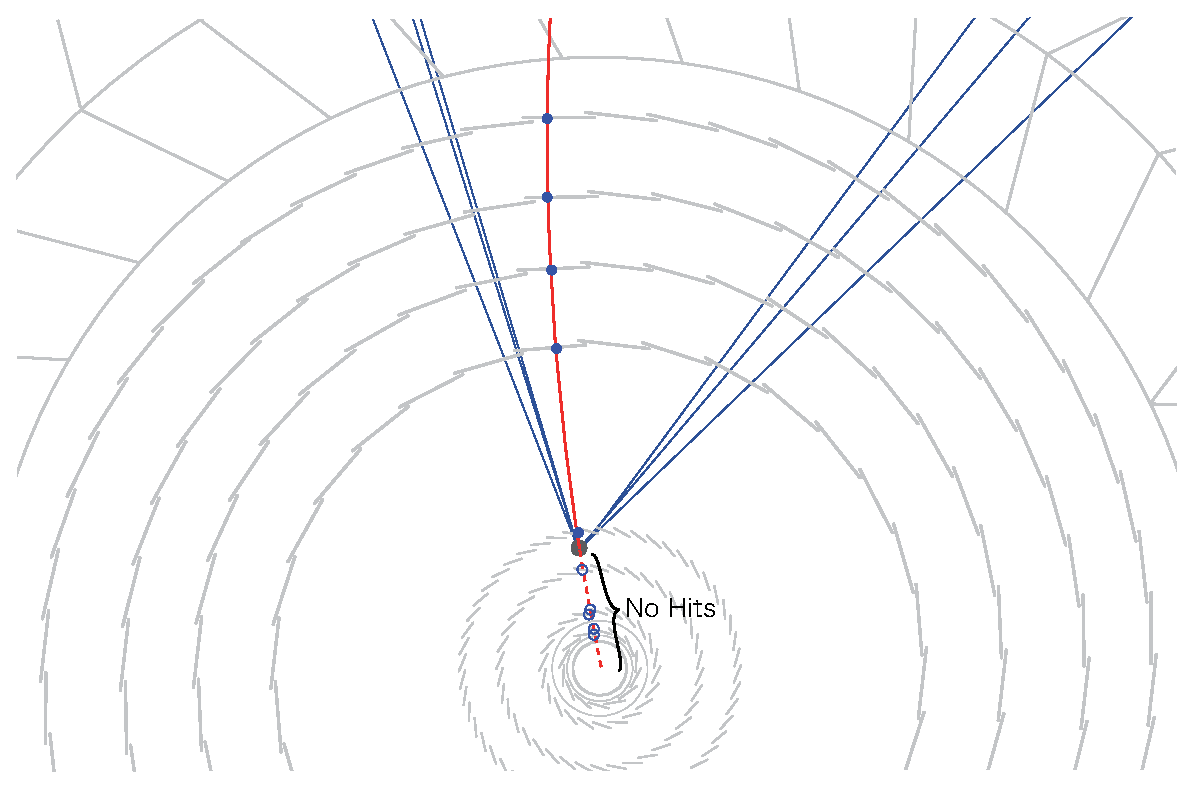
\includegraphics[width=0.5\textwidth]{figures/reattach}
%\caption{Illustration of track re-attachment. The red track is a candidate track to be associated to the displaced vertex, which was rejected in the track-seed selection step. The candidate track can be associated to the primary or pileup vertex, but the hit-pattern consistency check is applied.}
%\label{fig:reattach}
%\end{center}
%\end{figure}

\subsubsection{Final merging}
Vertices are finally forced to merge if the distance between the two vertices $D$ are closer than $(\alpha + \beta r)$ where $(\alpha,\beta)$ are the user-specified parameters ({\tt MergeFinalVerticesDist} and \\{\tt MergeFinalVerticesScaling} respectively). The coefficient $\beta$ was newly introduced in release {\tt 21}.


\subsubsection{Track re-attachment [new in {\tt r21}]}
Tracks that are not selected in the seed-track selection stage are not associated to any displaced vertices so far. It has been pointed that some of these tracks can be recovered and associated after the displaced vertices are found, and this feature was implemented in release {\tt 21}. The potential drawback of this step is to accidentally attaching irrelevant tracks or fake tracks.

Before re-attachment procedure starts, the vertex $\chi^{2}$ is optimised by running an iteration of detaching worst-associated tracks until the $\chi^{2}$ gets in a certain $\chi^{2}$-probability (specified by the job property). If the distance between the secondary vertex of interest and any of the hard-scatter or pileup primary vertices is smaller than the user-specified value (configurable by the job property {\tt associateMinDistanceToPV}), then re-attachment procedure is skipped.

All tracks in {\tt InDetTrackParticleContainer} is looped, then the tracks which are already used in any of secondary vertices at the point of loop are rejected. In addition, requirement to minimum \pt (the threshold specified by job property {\tt associatePtCut}), and to maximum track $\chi^{2}/N_{\rm dof}$ ({\tt associateChi2Cut}) are imposed. In addition, a similar requirement of the \emph{Classical} hit pattern in Section \ref{sec:ditrack} is applied. This hit pattern has however a relaxed requirement and only imposes requirement to outer layers than the vertex's transverse radius. For vertices within the innermost pixel layer, the requirement is reinforced to have hits in the closest two outer layers.

Once the track satisfies all the above criteria, the impact parameter with respect to the secondary vertex of interest is calculated, and if the track is close enough to the candidate vertex (both $d_{0}$ and $z_{0}$ significance to be smaller than user-specified values by {\tt associateMaxD0Signif} and {\tt associateMaxZ0Signif}), it is associated to the vertex and the vertex is refit with adding the track. At this point the variable {\tt is\_associated} is augmented to the track. Refitting is repeated for each track association attempt, and if fitting fails, the attachment of the track is skipped. Note that a track to be attached is allowed to be (already) associated to the primary or pileup vertices, but not allowed to be associated to multiple secondary vertices.

The criteria of which kind of tracks is eligible to be attached to the reconstructed vertices have some room of improvement with taking a balance between signal property enrichment and the fake vertices increase. The candidate vertex is searched in descending order of the track multiplicity, and track that are already used in some other displaced vertex are not associated anymore.



\subsubsection{Refitting and recording}
The reconstructed displaced vertices are finally stored as {\tt xAOD::Vertex}. The vertex $\chi^{2}/N_{\rm dof}$ can be optionally improved by detaching worst-matching tracks until the $\chi^{2}$ probability satisfies the specified criteria. After this procedure, if the vertex does not keep at least two originally selected tracks before re-attachment, it is dropped. Then the final displaced vertices are stored to the output {\tt xAOD::VertexContainer} named as {\tt VrtSecInclusive\_SecondaryVertices}. Simultaneously, augmentation to tracks used for final displaced vertices are made for e.g.~impact parameters with respect to the associated displaced vertex. In addition to the standard variables equipped in {\tt xAOD::Vertex}, several variables are augmented, as listed in Table \ref{tbl:auxdyn_vertices}. Similarly, additional augmentations are made to track particles on the course of vertex reconstruction, and these are listed in Table \ref{tbl:auxdyn_tracks}.

\begin{table}[htbp]
\caption{List of augmented variables to the vertices in {\tt VrtSecInclusive\_SecondaryVertices}.}
\centering
\scriptsize
\begin{tabular}{llp{10cm}}
\hline
\hline
name & type & description\\
\hline
{\tt vtx\_px} & {\tt float} & sum momenta $x$-component of tracks using track parameters with respect to the secondary vertex\\
{\tt vtx\_px} & {\tt float} & sum momenta $y$-component of tracks using track parameters with respect to the secondary vertex\\
{\tt vtx\_px} & {\tt float} & sum momenta $z$-component of tracks using track parameters with respect to the secondary vertex\\
{\tt vtx\_mass} & {\tt float} & sum momenta invariant mass of tracks using track parameters with respect to the secondary vertex where the charged pion mass is assumed for each track\\
{\tt vtx\_charge} & {\tt float} & sum charge of tracks\\
{\tt chi2\_core} & {\tt float} & the vertex $\chi^{2}$ before track re-attachment\\
{\tt ndof\_core} & {\tt float} & the vertex $N_{\rm dof}$ before track re-attachment\\
{\tt chi2\_assoc} & {\tt float} & the vertex $\chi^{2}$ after track re-attachment\\
{\tt ndof\_assoc} & {\tt float} & the vertex $N_{\rm dof}$ after track re-attachment\\
{\tt mass} & {\tt float} & almost identical to {\tt vtx\_mass} but explicitly re-calculating the mass using tracking parameters and assuming the charged pion mass for all tracks\\
{\tt mass\_e} & {\tt float} & almost identical to {\tt vtx\_mass} but explicitly re-calculating the mass using tracking parameters and assuming the electron mass for all tracks\\
{\tt mass\_proton} & {\tt float} & almost identical to {\tt vtx\_mass} but explicitly re-calculating the mass using tracking parameters and assuming the proton mass for all tracks\\
{\tt mass\_selectedTracks} & {\tt float} & same as {\tt mass} but only using the selected tracks (not using the attached tracks)\\
{\tt minOpAng} & {\tt float} & the maximum of cosine of the opening angles between all track pairs within the vertex, using track parameters with respect to the secondary vertex\\
{\tt num\_trks} & {\tt int} & the number of tracks comprising the vertex. This should be identical to {\tt xAOD::Vertex::nTrackParticles()}.\\
{\tt num\_selectedTracks} & {\tt int} & the number of selected tracks within the comprising tracks.\\
{\tt num\_associatedTracks} & {\tt int} & the number of associated tracks within the comprising tracks. The sum of {\tt num\_selectedTracks} and {\tt num\_associatedTracks} should be equal to {\tt num\_trks}.\\
{\tt dCloseVrt} & {\tt float} & the significance of the distance to the closest secondary vertex\\
\hline
\hline
\end{tabular}
\label{tbl:auxdyn_vertices}
\end{table}%

\begin{table}[htbp]
\caption{List of augmented variables to {\tt xAOD::TrackParticle}. Note that the container of the tracks is not always {\tt InDetTrackParticleContainer}. For example, when the electron-associated tracks are used, the track can be stored in other containers like {\tt GSF...}. All variable names may have a suffix string which is specified by the user job property {\tt AugmentingVersionString} in order to label for which secondary vertex container the variable is created. The variables latter than {is\_svtrk\_final} are all referring to the final reconstruction vertices (i.e. the vertex instances in {\tt VrtSecInclusive\_SecondaryVertices}, and there are no corresponding augmentations for the intermediate step vertices.}
\centering
\scriptsize
\begin{tabular}{llp{11cm}}
\hline
\hline
name & type & description\\
{\tt is\_selected} & {\tt char} & augmented and stored {\tt true} if the track selection algorithm selected the track. This does not mean that such a track is indeed used in the reconstructed secondary vertices.\\
{\tt is\_associated} & {\tt char} & augmented and stored {\tt true} if the track re-attachment algorithm attaches the track to the vertex. This does not mean that such a track is used in the reconstructed secondary vertices; the improvement of vertex $\chi^{2}$ function may detach the track later.\\
{\tt is\_svtrk\_final} & {\tt char} & augmented and stored {\tt true} if the track is used for the final secondary vertices.\\
{\tt d0\_wrtSV} & {\tt float} & the value of $d_{0}$ with respect to the reconstructed vertex. augmented and stored if the track is used for the final secondary vertices.\\
{\tt z0\_wrtSV} & {\tt float} & the value of $z_{0}$ with respect to the reconstructed vertex. augmented and stored if the track is used for the final secondary vertices.\\
{\tt pt\_wrtSV} & {\tt float} & the value of \pt with respect to the reconstructed vertex. augmented and stored if the track is used for the final secondary vertices.\\
{\tt eta\_wrtSV} & {\tt float} & the value of $\eta$ with respect to the reconstructed vertex. augmented and stored if the track is used for the final secondary vertices.\\
{\tt phi\_wrtSV} & {\tt float} & the value of $\phi$ with respect to the reconstructed vertex. augmented and stored if the track is used for the final secondary vertices.\\
{\tt errd0\_wrtSV} & {\tt float} & the square of $d_{0}$ uncertainty with respect to the reconstructed vertex. augmented and stored if the track is used for the final secondary vertices.\\
{\tt errz0\_wrtSV} & {\tt float} & the square of $z_{0}$ uncertainty with respect to the reconstructed vertex. augmented and stored if the track is used for the final secondary vertices.\\
{\tt errP\_wrtSV} & {\tt float} & the square of $q/p$ uncertainty with respect to the reconstructed vertex. augmented and stored if the track is used for the final secondary vertices.\\
{\tt chi2\_toSV} & {\tt float} & the $\chi^{2}$ value (goodness of association) of the track to the reconstructed vertex. augmented and stored if the track is used for the final secondary vertices.\\
\hline
\hline
\end{tabular}
\label{tbl:auxdyn_tracks}
\end{table}%

\subsubsection{Additional augmentation to leptons}
After all vertex reconstruction is done, optionally, the track parameters of the tracks associated to leptons (muons or electrons) with respected to the reconstructed secondary vertices can be calculated, and the values are augmented to the lepton instances.

%-------------------------------------------------------------------------------
\subsection{Configuring {\tt VrtSecInclusive} in {\tt athena}}
\label{sec:config}
%-------------------------------------------------------------------------------

\subsubsection{Configuring {\tt jobOption}}
{\tt VrtSecInclusive/share/VrtSecInclusive\_DV\_Configuration.py} is a good example of how to use {\tt VrtSecInclusive} within {\tt athena}. In general the reconstruction algorithm does not have downstream dependencies, then the algorithm instance can be appended in the last of the {\tt AthAlgSequence} queue:

\begin{scriptsize}
\begin{verbatim}
...
from AthenaCommon.AlgSequence import AlgSequence
topSequence = AlgSequence()
from VrtSecInclusive.VrtSecInclusive import VrtSecInclusive
...
VrtSecInclusive_InDet = VrtSecInclusive("VrtSecInclusive_InDet")
topSequence.insert(-1, VrtSecInclusive_InDet)
...
\end{verbatim}
\end{scriptsize}

Multiple {\tt VrtSecInclusive} instances with different configurations can run within a single reconstruction. The instance names need to be varied in this case:

\begin{scriptsize}
\begin{verbatim}
...
VrtSecInclusive_InDet = VrtSecInclusive("VrtSecInclusive_InDet")
VrtSecInclusive_leptons  = VrtSecInclusive("VrtSecInclusive_leptons")
...
topSequence.insert(-1, VrtSecInclusive_InDet)
topSequence.insert(-1, VrtSecInclusive_leptons)
...
\end{verbatim}
\end{scriptsize}

The augmented variables (see previous section) to the {\tt xAOD::TrackParticles} will produce name conflict if multiple {\tt VrtSecInclusive} algorithms run. Therefore, these need to be resolved by adding adequate suffices. The job property {\tt AugmentingVersionString} is used for this purpose:

\begin{scriptsize}
\begin{verbatim}
...
VrtSecInclusive_InDet.AugmentingVersionString   = ""
...
VrtSecInclusive_leptons.AugmentingVersionString = "_Leptons"
...
\end{verbatim}
\end{scriptsize}

\subsubsection{Storing containers}
In order to ensure the output containers are saved, the snippet like the following may be needed (the stream name would need to be changed accordingly depending on which transform step you are working on):
\begin{scriptsize}
\begin{verbatim}
StreamAOD.ItemList+=["xAOD::TrackParticleContainer#*"]
StreamAOD.ItemList+=["xAOD::TrackParticleAuxContainer#*"]
StreamAOD.ItemList+=["xAOD::VertexContainer#*"]
StreamAOD.ItemList+=["xAOD::VertexAuxContainer#*"]
\end{verbatim}
\end{scriptsize}

\subsubsection{Detector condition loading}
In case of the {\tt VrtSecInclusive} reconstruction to take place in {\tt RAWtoESD}, the inner detector conditions are loaded by default and user does not need any additional treatment. For using it in {\tt ESDtoAOD} or {\tt AODtoDAOD} this is not the case. The appropriate job option needs to be figured out.


%-------------------------------------------------------------------------------
\subsection{Performance}
\label{sec:result}
%-------------------------------------------------------------------------------

In this section, the performance of vertex reconstruction with {\tt VrtSecInclusive} optimised for the production of {\tt AOD\_RPVLL} in release {\tt 21} is evaluated and discussed. The reconstruction was performed using {\tt 21.0.50} on the {\tt RAWtoESD} process of {\tt Reco\_tf.py} for data, and {\tt AtlasDerivation, 20.7.9.7} on the {\tt ADOtoDAOD} process of the {\tt DAOD\_SUSY15} derivation for the MC samulation samples, with overriding the {\tt VrtSecInclusive} package by the identical test implementation for both cases.

\subsubsection{Benchmark configuration}
The following configuration is the one implemented in\\{\tt VrtSecInclusive/share/VrtSecInclusive\_DV\_Configuration.py} as the instance\\ {\tt VrtSecInclusive\_InDet} in release {\tt 21}.

\paragraph{Track selection for vertex seeding}
The job properties other than specified are all set to the default value.
{\tt do\_PVvetoCut} is enabled; {\tt do\_d0Cut}, {\tt do\_z0Cut}, {\tt do\_d0errCut}, {\tt do\_z0errCut} , {\tt do\_d0signifCut}, {\tt do\_z0signifCut} are all disabled; {\tt doTRTPixCut} is enabled; {\tt DoSAloneTRT} is disabled.

The parameters are set as follows: {\tt CutPixelHits = 0}; {\tt CutSctHits = 2}; {\tt CutSharedHits = 2}; {\tt TrkPtCut = 1000.}\,[MeV]; {\tt TrkChi2Cut = 50}; {\tt SelTrkMaxCutoff = 2000}.

\paragraph{Vertex reconstruction}
{\tt doPVcompatibilityCut} is diabled; {\tt RemoveFake2TrkVrt} is enabled; {\tt CheckHitPatternStrategy} used is {\tt 'ExtrapolationAssist'}; {\tt doReassembleVertices} is enabled; {\tt doMergeByShuffling} is enabled; {\tt doMergeFinalVerticesDistance} is enabled; {\tt doAssociateNonSelectedTracks} is enabled; {\tt doFinalImproveChi2} is enabled.

The parameters are set as follows: {\tt twoTrkVtxFormingD0Cut = 2.0}\,[mm];\\
{\tt SelVrtChi2Cut = 5} ($\chi^{2}/N_{\rm dof}$); {\tt mergeByShufflingAllowance = 10.}\,[sigma];\\
{\tt associatePtCut = 1000.}\,[\MeV];\\
{\tt associateMaxD0Signif = 5.}\,[sigma]; {\tt associateMaxZ0Signif = 5.}\,[sigma];\\
{\tt MergeFinalVerticesDist = 1.}\,[mm]; {\tt MergeFinalVerticesScaling = 0.001}\,[1/mm];\\ {\tt improveChi2ProbThreshold = 0.0001}.

\paragraph{Other configurations}
{\tt doAugmentDVimpactParametersToMuons} is enabled; {\tt doAugmentDVimpactParametersToElectrons} is enabled.

\subsubsection{Signal efficiency and reconstructed properties}
The performance test was carried out for a couple of {\tt mc15\_13TeV} {\tt AOD} samples of long-lived $R$-hadrons, with each of them having several thousands events as listed in Table \ref{tbl:mc_samples}. These {\tt AOD} samples were created in {\tt r20.7} with a large-$d_{0}$ tracking option of $\pt>500~\MeV$ up to $|d_{0}|<300~{\rm mm}$\footnote{For release {\tt 21} reconstruction the \pt threshold is raised to 900~\MeV.}. The newly developed {\tt VrtSecInclusive} for {\tt rel21} was specially compiled with {\tt AtlasDerivation, 20.7.9.7}. The algorithm was run on the process {\tt AODtoDAOD} along the production of {\tt DAOD\_SUSY15}.

\paragraph{Signal efficiency}
These efficiencies described here are measured by a distance-based vertex truth matching. For a given truth vertex, if any of the reconstructed vertices at the given step satisfies either the truth--reco distance to be less than 2 mm or the significance of the distance is less than 10 sigma, then the truth vertex is tagged as \emph{reconstructed}. Here, the threshold of the distance or significance is taken quite wide to avoid the leaking of the matching due to the long-tailed vertex resolution. The frequency of having irrelevant vertices other than the truth vertex is assumed small and ignored in this relatively simple estimation.

A few efficiencies are defined to probe different aspects of the reconstruction features as follows;
\begin{description}
\item{\emph{Vertex-seeding efficiency}, $\varepsilon_{\rm seed}$}: The denominator is all truth vertices of interest. The numerator is the number of truth vertices which have at least one reconstructed vertex at the di-track vertex finding step before applying any cut. Track pairs which do not satisfy the $d_{0}^{\rm init}$ or $z_{0}^{\rm init}$ filter are not counted. This efficiency approximately probes the net effect of track reconstruction and selection efficiency for the given vertex.

\item{\emph{Algorithmic reconstruction efficiency}, $\varepsilon_{\rm alg}$}: The denominator is the numerator of the vertex-seeding efficiency, and the numerator is the number of truth vertices which have (at least one) corresponding reconstructed vertices at the final reconstruction output.

\item{\emph{Total reconstruction efficiency}, $\varepsilon_{\rm tot}$}: The denominator is all truth vertices of interest. The numerator is the number of truth vertices which have (at least one) corresponding reconstructed vertices at the final reconstruction output. This is equal to the product of the vertex-seeding efficiency and the algorithmic reconstruction efficiency.
\end{description}

Figure \ref{fig:nmatch_eff_exAssist} shows radius-binned efficiencies of the above three for $R$-hadron decays. The vertex-seeding efficiency $\varepsilon_{\rm seed}$ ramps up around $r$ of 1--2 mm then gradually degrades up to $r$ of around 200 mm, then drops down quickly towards $r$ of around 300 mm, which meets approximately the first SCT barrel layer. The cutoff at the small radii around 1--2 mm is generally determined by requirement to the transverse impact parameter or veto of tracks associated to the primary vertices, while the cutoff at the larger radii is mostly determined by the tracking efficiency loss\footnote{For this argument, readers are guided to read the large-radius tracking PUB note ATL-PHYS-PUB-2017-014.}. The algorithmic efficiency $\varepsilon_{\rm alg}$ should ideally be kept as close as~1, but some inefficiencies are present. Large part of inefficiencies are due to requirement of the hit-pattern to the constituent tracks at the stage of di-track finding.

The case of \{ $m(\gluino) = 2~\TeV$, $m(\tilde{\chi}_{1}^{0}) = 100~\GeV$ \} has generally higher algorithmic efficiency compared to \{ $m(\gluino) = 2~\TeV$, $m(\tilde{\chi}_{1}^{0}) = 1.9~\TeV$ \}, and this is mostly due to large track multiplicity and statistically the likelihood of that some pair combinations of the selected tracks pass the criteria is relatively higher than the other case. The feature of reconstruction efficiency which strongly depends on how many selected tracks are present for the given truth vertex is represented in Figure \ref{fig:effMult}. The efficiency at particularly small multiplicity is not satisfactory, but the source of inefficiency is mostly the hit pattern requirement for rejecting fake vertices. It is desired to have a more sophisticated classification in order to save more of small track-multiplicity vertices. It is observed that the radial decay position dependence of the efficiency as a function of multiplicity is not very strong.

\begin{table}[tbp]
\caption{default}
\centering
\scriptsize
\begin{tabular}{llrp{9.6cm}}
\hline
\hline
DSID & format & events & description\\
\hline
{\tt mc15\_13TeV.402735}& {\tt AOD (r20.7)} & 5k   & $m(\gluino) = 2~\TeV$, $m(\tilde{\chi}_{1}^{0}) = 100~\GeV$, $\tau(\gluino) = 1~{\rm ns}$; large-$d_{0}$ tracking ($\pt > 500~\MeV$)\\
{\tt mc15\_13TeV.403087}& {\tt AOD (r20.7)} & 9.8k & $m(\gluino) = 2~\TeV$, $m(\tilde{\chi}_{1}^{0}) = 1.9~\TeV$, $\tau(\gluino) = 1~{\rm ns}$; large-$d_{0}$ tracking ($\pt > 500~\MeV$)\\
{\tt data16\_13TeV.00310249} & {\tt DRAW\_RPVLL (r21)} & 3k  & {\tt physics\_Main}, randomly selected 20 files; large-$d_{0}$ tracking ($\pt > 900~\MeV$)\\
\hline
\hline
\end{tabular}
\label{tbl:mc_samples}
\end{table}%

\begin{figure}[t]
\begin{center}
\subfigure[$m(\gluino) = 2~\TeV$, $m(\tilde{\chi}_{1}^{0}) = 100~\GeV$]{ 
  \label{fig:nmatch_eff_exAssist_mc15_13TeV.402735}
  \includegraphics[width=0.48\textwidth]{figures/nmatch_eff_exAssist_mc15_13TeV_402735.pdf}
}
\subfigure[$m(\gluino) = 2~\TeV$, $m(\tilde{\chi}_{1}^{0}) = 1.9~\TeV$]{ 
  \label{fig:nmatch_eff_exAssist_mc15_13TeV.403087} 
  \includegraphics[width=0.48\textwidth]{figures/nmatch_eff_exAssist_mc15_13TeV_403087.pdf}
}
\caption{Vertex-seeding, algorithmic, and total reconstruction efficiency for $R$-hadron decay MC simulation samples as a function of the decay transverse radius.}
\label{fig:nmatch_eff_exAssist}
\end{center}
\end{figure}

\begin{figure}[t]
\begin{center}
\subfigure[$m(\gluino) = 2~\TeV$, $m(\tilde{\chi}_{1}^{0}) = 100~\GeV$]{ 
  \label{fig:effMult402735}
  \includegraphics[width=0.48\textwidth]{figures/effMult_402735}
}
\subfigure[$m(\gluino) = 2~\TeV$, $m(\tilde{\chi}_{1}^{0}) = 1.9~\TeV$]{ 
  \label{fig:effMult_403087} 
  \includegraphics[width=0.48\textwidth]{figures/effMult_403087}
}
\caption{Total reconstruction efficiency as a function of multiplicity of the selected tracks associated to the truth vertex.}
\label{fig:effMult}
\end{center}
\end{figure}


\paragraph{Reconstruction of kinematic properties}
For searches which uses displaced vertices as the signature, not only \emph{how much} the signal vertices are reconstructed, but also \emph{how well} they are reconstructed are equally important. Reconstruction of the track multiplicity and the invariant mass is particularly important, since these two variables are used as the discriminants to define the signal region. The following two fractions are defined:

\begin{description}
\item{\emph{Visible multiplicity fraction}}: The denominator is the number of outgoing truth particles of the truth vertex which satisfy $\pt>1~\GeV$ (the fiducial cut). The numerator is the multiplicity of the tracks of the truth-matched reconstructed vertex.
\item{\emph{Visible mass fraction}}: The denominator is the invariant mass formed from outgoing truth particles of the truth vertex which satisfy $\pt>1~\GeV$ (the fiducial cut). The numerator is the invariant of the tracks of the truth-matched reconstructed vertex.
\end{description}

Figure \ref{fig:vismult_fraction} and \ref{fig:vismass_fraction} show the visible multiplicity fraction and mass fraction of $R$-hadron decays as a function of the decay transverse radius respectively. It is clearly shown that both of multiplicity and mass are reconstructed quite accurately for the range $r\lesssim 50$ mm, while for outer radii the properties are gradually lossed. The sharpness of the fraction is better for the smaller multiplicity case of \{ $m(\gluino) = 2~\TeV$, $m(\tilde{\chi}_{1}^{0}) = 1.9~\TeV$ \}, and there would be more room of improvement in the track re-attachment feature for the future.

Figure \ref{fig:reattachment_effect} additionally demonstrates the importance of the track re-attachment function for the recovery of the vertex property. The orange bullets are the average multiplicity of the tracks, while the light blue bullets show the one after track re-attachment. Remarkably the trend of the blue bullets is almost catching up that of reconstructed tracks (gray squares) except $r\lesssim 2$ mm. This improvement of the recovery of the vertex properties helps increase the yield of the signal vertices in the signal region significantly.

\begin{figure}[t]
\begin{center}
\subfigure[$m(\gluino) = 2~\TeV$, $m(\tilde{\chi}_{1}^{0}) = 100~\GeV$]{ 
  \label{fig:nmatch_eff_exAssist_mc15_13TeV.402735}
  \includegraphics[width=0.48\textwidth]{figures/mult_402735_sample1}
}
\subfigure[$m(\gluino) = 2~\TeV$, $m(\tilde{\chi}_{1}^{0}) = 1.9~\TeV$]{ 
  \label{fig:nmatch_eff_exAssist_mc15_13TeV.403087} 
  \includegraphics[width=0.48\textwidth]{figures/mult_403087_sample1}
}
\caption{Visible multiplicity fraction as a function of $R$-hadron decay radius.}
\label{fig:vismult_fraction}
%\end{center}
%\end{figure}

%\begin{figure}[t]
%\begin{center}
\subfigure[$m(\gluino) = 2~\TeV$, $m(\tilde{\chi}_{1}^{0}) = 100~\GeV$]{ 
  \label{fig:nmatch_eff_exAssist_mc15_13TeV.402735}
  \includegraphics[width=0.48\textwidth]{figures/mass_402735_sample1}
}
\subfigure[$m(\gluino) = 2~\TeV$, $m(\tilde{\chi}_{1}^{0}) = 1.9~\TeV$]{ 
  \label{fig:nmatch_eff_exAssist_mc15_13TeV.403087} 
  \includegraphics[width=0.48\textwidth]{figures/mass_403087_sample1}
}
\caption{Visible mass fraction as a function of $R$-hadron decay radius.}
\label{fig:vismass_fraction}
\end{center}
\end{figure}


\begin{figure}[tbp]
\begin{center}
\subfigure[$m(\gluino) = 2~\TeV$, $m(\tilde{\chi}_{1}^{0}) = 100~\GeV$]{ 
  \label{fig:nmatch_eff_exAssist_mc15_13TeV.402735}
  \includegraphics[width=0.48\textwidth]{figures/multiplicity_402735_1}
}
\subfigure[$m(\gluino) = 2~\TeV$, $m(\tilde{\chi}_{1}^{0}) = 1.9~\TeV$]{ 
  \label{fig:nmatch_eff_exAssist_mc15_13TeV.403087} 
  \includegraphics[width=0.48\textwidth]{figures/multiplicity_403087_1}
}
\caption{Average track or charged truth particle multiplicity of $R$-hadron decay products of $\pt>1~{\rm GeV}$ as a function of the decay transverse position. After re-attachment of the tracks, most of the reconstructed tracks are associated to the vertex.}
\label{fig:reattachment_effect}
\end{center}
\end{figure}

\paragraph{Track purity}
Some tracks associated to the reconstructed vertex might not be truly originated from the vertex. It is of interests to also check the purity of the tracks comprising the signal vertex. In order to evaluate this, tracks are classified into the following five categories:
\begin{description}
\item {\emph{Truth}}: the truth particle matched to the reconstructed track is an outgoing particle of the truth-matched vertex.
\item {\emph{Primary}}: the truth particle matched to the reconstructed track is originated from the either hard-scatter or pileup primary vertices.
\item {\emph{Around}}: the truth particle matched to the reconstructed track is not an outgoing particle of the matched true vertex, but it is originated from some other vertex which are around the true vertex of interest within 2 mm. Some of the ``around'' category tracks may be considered as a part of truth, in particular such ``around`` vertices may be cascade decays of the children products of the truth decay.
\item {\emph{Away}}: the truth particle matched to the reconstructed track is not an outgoing particle of the matched true vertex, but it is originated from some other vertex which are far from the true vertex of interest more than 2 mm.
\item {\emph{Fake or pileup}}: the truth particle matched to the reconstructed track is not found. Note that both primary and secondary tracks which are sourced to pileup vertices are classified in this category due to not recording the truth information in the MC simulation.
\end{description}

The composition of the track truth categories for the reconstructed $R$-hadron decay vertices in Figure \ref{fig:Rhadron_trackType}. The accidental attachment of primary and fake vertices are quite well suppressed in average, while a few to ten percent of contamination of ``around'' and ``away'' vertices are present. The purity of the truth tracks at this level would be considered quite satisfiable.

\begin{figure}[tbp]
\begin{center}
\subfigure[$m(\gluino) = 2~\TeV$, $m(\tilde{\chi}_{1}^{0}) = 100~\GeV$]{ 
  \label{fig:nmatch_eff_exAssist_mc15_13TeV.402735}
  \includegraphics[width=0.48\textwidth]{figures/Rhadron_trackType_402735}
}
\subfigure[$m(\gluino) = 2~\TeV$, $m(\tilde{\chi}_{1}^{0}) = 1.9~\TeV$]{ 
  \label{fig:nmatch_eff_exAssist_mc15_13TeV.403087} 
  \includegraphics[width=0.48\textwidth]{figures/Rhadron_trackType_403087}
}
\caption{The composition of the track truth categories for the reconstructed $R$-hadron decay vertices.}
\label{fig:Rhadron_trackType}
\end{center}
\end{figure}

\paragraph{Vertex resolution}
Something to be noted down... e.g.~non-gaussianity.

\begin{figure}[tbp]
\begin{center}
\subfigure[Residual distribution example]{ 
  \label{fig:res_r_4}
  \includegraphics[width=0.48\textwidth]{figures/res_r_4}
}
\subfigure[Resolution vs $r_{\rm vertex}$]{ 
  \label{fig:res_402735} 
  \includegraphics[width=0.48\textwidth]{figures/res_402735}
}
\caption{\subref{fig:res_r_4} Example of the residual distribution of the radial vertex position with respect to the matched true vertex of $R$-hadron decays of \{ $m(\gluino) = 2~\TeV$, $m(\tilde{\chi}_{1}^{0}) = 100~\GeV$ \}. \subref{fig:res_402735} The radial ($r$), longitudinal ($z$) and azimuthal ($r_{\rm vertex}\times\phi$) vertex resolution for the case of \{ $m(\gluino) = 2~\TeV$, $m(\tilde{\chi}_{1}^{0}) = 100~\GeV$ \}. The resolution is defined as the 1-sigma of the iterative fitting of the core $\pm2.5\sigma$ range of the residual distribution with a coaxial double gaussian (taking the narrower sigma of the two gaussians).}
\label{fig:Rhadron_trackType}
\end{center}
\end{figure}

\paragraph{Split vertices rate}
The split vertices may be produced due to the long-tail behaviour of the vertex resolution when the track multiplicity is relatively high. The rate of split vertices can be suppressed by the various vertex merging recipes described in Section \ref{sec:merging}. For the case of $m(\gluino) = 2~\TeV$, $m(\tilde{\chi}_{1}^{0}) = 100~\GeV$, $\tau(\gluino) = 1~{\rm ns}$ where around 35 reconstructed tracks are present on a vertex, the achieved split rate is around 0.3\%, while it is more than 10\% without merging methods.

\subsubsection{Data yield}
Here, vertex yields and properties are planned to be compared between release {\tt 20.7} and the up-to-date {\tt VrtSecInclusive}. Also, there should be a comment on the treatment of disabled pixel modules -- for this, I would need to wait for a test production of the {\tt DAOD\_RPVLL}.

\subsubsection{CPU consumption and data size}

\begin{table}[htbp]
\centering
\caption{Average CPU time consumption per event as a function of reconstruction step for different event samples. The concrete step is as follows. a) di-track vertex finding, b) $n$-track vertex finding (incompatible graph), c) vertex re-arrangement, d) re-assembling, e) vertex merging by shuffling, f) forced merging by distance, g) track re-attachment, h) refitting and storing.}
\begin{tabular}{lrrrrrrrrrr}
\hline
\hline
Step & a & b & c & d & e & f & g & h & sum &\\
\hline
{\tt mc15\_13TeV.402735} & 199.7 & 14.7 & 17.4 & 1.1 & 1.3 & 0.0 & 24.6 & 9.6 & 268.3 & [ms/event]\\
{\tt mc15\_13TeV.404087} & 51.9 & 2.2 & 0.7 & 0.4 & 0.2 & 0.0 & 6.3 & 2.7 & 64.3 & [ms/event]\\
{\tt data16\_13TeV.00310249} & 340.5 & 3.8 & 0.1 & 0.0 & 1.1 & 0.0 & 24.7 & 5.2 & 375.3 & [ms/event]\\
\hline
\hline
\end{tabular}
\label{tbl:default}
\end{table}%

Need also a table for the data size...

\subsection{Known issues and future potential}
Should describe where {\tt VrtSecInclusive} has weakness and how we could possibly improve in the future.
\begin{itemize}
\item performance to be checked: pileup dependence. Fake yield may explode?
\item how can we better classify fake vertices from signal? Is machine-learning helpful?
\item how much can we recover the non-attached tracks?
\item not great efficiency for small track multiplicity... how it is possible to recover the efficiency without huge increase of fakes?
\item how to reconstruct vertices very close to the primary vertex without huge increase of fakes?
\item lepton-only DV reconstruction... would it be useful?
\item do we need to think of re-weighting the tracks (like adaptive fitting?)
\item how much can we reduce the CPU consumption?
\end{itemize}


%-------------------------------------------------------------------------------
\subsection{Conclusion}
\label{sec:conclusion}
%-------------------------------------------------------------------------------
{\tt VrtSecInclusive} is not yet conclusive!

%-------------------------------------------------------------------------------
% If you use biblatex and either biber or bibtex to process the bibliography
% just say \printbibliography here
\printbibliography
% If you want to use the traditional BibTeX you need to use the syntax below.
%\bibliographystyle{bib/bst/atlasBibStyleWithTitle}
%\bibliography{VrtSecInclusive,bib/ATLAS,bib/CMS,bib/ConfNotes,bib/PubNotes}
%-------------------------------------------------------------------------------

%-------------------------------------------------------------------------------
% Print the list of contributors to the analysis
% The argument gives the fraction of the text width used for the names
%-------------------------------------------------------------------------------
%\clearpage
%\PrintAtlasContribute{0.30}


